\titledquestion{Dijkstra's Algorithm}[4]

Given the following weighted graph, run Dijkstra's algorithm by considering $A$ as the source vertex. Write down the vertex you select and update current distance \texttt{dis[i]} of all vertices in each iteration.

\vspace{1cm}

\begin{figure}[htbp]
    \centering
    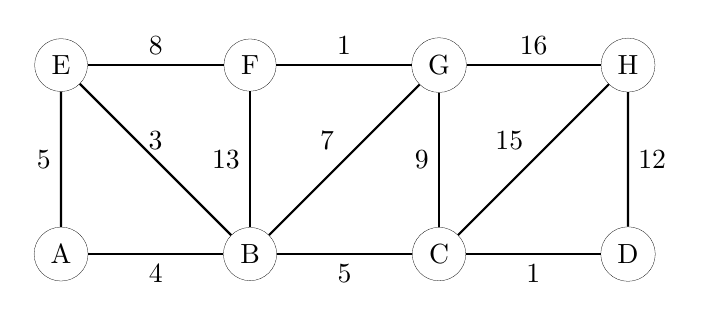
\begin{tikzpicture}
    [thick,scale=0.8, every node/.style={scale=1}]
    %		\node[circle] (n0){A};
    \node[circle, draw, line width=0.1pt] (a) at (-4.5,0){A};
    \node[circle, draw, line width=0.1pt] (b) at (-1.5,0){B};
    \node[circle, draw, line width=0.1pt] (c) at (1.5,0){C};
    \node[circle, draw, line width=0.1pt] (d) at (4.5,0){D};
    \node[circle, draw, line width=0.1pt] (e) at (-4.5,3){E};
    \node[circle, draw, line width=0.1pt] (f) at (-1.5,3){F};
    \node[circle, draw, line width=0.1pt] (g) at (1.5,3){G};
    \node[circle, draw, line width=0.1pt] (h) at (4.5,3){H};
    \draw[-] (a) to node[below]{4} (b);
    \draw[-] (a) to node[left]{5} (e);
    \draw[-] (b) to node[below]{5} (c);
    \draw[-] (b) to node[above]{3} (e);
    \draw[-] (b) to node[left]{13} (f);
    \draw[-] (b) to node[above left]{7} (g);
    \draw[-] (c) to node[below]{1} (d);
    \draw[-] (c) to node[left]{9} (g);
    \draw[-] (c) to node[above left]{15} (h);
    \draw[-] (d) to node[right]{12} (h);
    \draw[-] (e) to node[above]{8} (f);
    \draw[-] (f) to node[above]{1} (g);
    \draw[-] (g) to node[above]{16} (h);
    \end{tikzpicture}
\end{figure}


\begin{table}[htbp]
    \begin{center}  
        \begin{tabular}{|l|c|c|c|c|c|c|c|c|c| p{3cm}|}  
            \hline  
            & vertex & \texttt{dis[A]} & \texttt{dis[B]} & \texttt{dis[C]} & \texttt{dis[D]} & \texttt{dis[E]} & \texttt{dis[F]} & \texttt{dis[G]} & \texttt{dis[H]}\\ \hline  
            initial 	& / & 0 &$\infty$&$\infty$&$\infty$&$\infty$&$\infty$&$\infty$&$\infty$\\ \hline
            
            iteration 1 & & & & & & & & & \\ \hline    
            iteration 2 & & & & & & & & & \\ \hline    
            iteration 3 & & & & & & & & & \\ \hline    
            iteration 4 & & & & & & & & & \\ \hline    
            iteration 5 & & & & & & & & & \\ \hline    
            iteration 6 & & & & & & & & & \\ \hline    
            iteration 7 & & & & & & & & & \\ \hline    
            iteration 8 & & & & & & & & & \\ \hline    
            
            
        \end{tabular}  
    \end{center}  
\end{table}
